\documentclass[tikz,border=8pt]{standalone}
\usepackage{ctex}
\usepackage{amsmath,amssymb,bm}
\usetikzlibrary{arrows.meta,calc,decorations.pathmorphing,patterns,positioning,angles,quotes}
\definecolor{ink}{RGB}{28,41,56}
\definecolor{blue}{RGB}{35,91,168}
\definecolor{orange}{RGB}{218,112,24}
\definecolor{green}{RGB}{38,137,92}
\definecolor{red}{RGB}{190,51,51}
\tikzset{
  line cap=round,line join=round,
  axis/.style={->,very thick,ink},
  body/.style={very thick,draw=ink},
  curve/.style={very thick,draw=blue},
  rope/.style={very thick,draw=blue},
  ropeb/.style={very thick,draw=orange},
  vec/.style={-{Latex[length=2.5mm]},very thick,draw=blue},
  force/.style={-{Latex[length=2.5mm]},very thick,draw=red},
  guide/.style={draw=ink!45,dashed},
  dim/.style={{Latex[length=2mm]}-{Latex[length=2mm]},draw=ink!75},
  mass/.style={circle,draw=ink,very thick,fill=white,minimum size=7mm,inner sep=0pt}
}

\tikzset{mass/.style={circle,draw,fill=white,minimum size=7mm},curve/.style={very thick,blue},rope/.style={very thick,blue},ray/.style={very thick,blue,-{Latex}},impulse/.style={very thick,orange,-{Latex}},resistor/.style={thick,decorate,decoration={zigzag,segment length=3mm,amplitude=1mm}}}
\begin{document}
% 1 question-01
\begin{tikzpicture}[x=1cm,y=1cm]
  \draw[body] (-4.8,0)--(4.8,0);
  \foreach \x in {-4.5,-4.1,...,4.5}{\draw[ink!45] (\x,0)--++(-.25,-.18);}
  \draw[body] (-.25,0)--(-.25,4.4) (.25,0)--(.25,4.4);
  \node[mass] (A) at (0,3.75) {$A$};
  \node[mass] (B) at (0,.36) {$B$};
  \draw[very thick,orange] (A)--(B);
  \draw[dim] (.65,.36)--(.65,3.75) node[midway,right] {$L$};
  \node[align=center] at (0,-.75) {$A$ 沿竖直槽运动，$B$ 沿水平面运动\\初始时轻杆竖直};
\end{tikzpicture}

% 2 solution-01
\begin{tikzpicture}[x=1cm,y=1cm]
  \draw[body] (-5.4,-1.5)--(5.4,-1.5);
  \draw[body] (-4.25,-1.5)--(-4.25,3.8);
  \coordinate (O) at (-4.25,-1.5);
  \coordinate (A) at (-4.25,2.25);
  \coordinate (B) at (.35,-1.5);
  \draw[very thick,orange] (A)--(B);
  \node[mass] at (A) {$A$}; \node[mass] at (B) {$B$};
  \draw[guide] (A)--(-4.25,-1.5) (B)--(-4.25,-1.5);
  \pic[draw=ink,->,"$\theta$",angle radius=10mm,angle eccentricity=1.28]
    {angle=O--A--B};
  \draw[vec] ($(A)+(-.65,0)$)--++(0,-1.25) node[left] {$v_A$};
  \draw[vec] (B)--++(1.45,0) node[above] {$v_B$};
  \node[align=left,anchor=west] at (1.6,2.55)
    {$y_A=L\cos\theta$\\[2pt]
     $x_B=L\sin\theta$\\[2pt]
     $v_A=L\sin\theta\,\dot\theta$\\[2pt]
     $v_B=L\cos\theta\,\dot\theta$};
  \node[align=center] at (0,-2.25)
    {同一根刚杆给出速度约束；$B$ 的动能极大时杆内力为零};
\end{tikzpicture}

% 3 question-02
\begin{tikzpicture}[x=1cm,y=1cm]
  \draw[body] (-4.8,2.5)--(4.8,2.5);
  \coordinate (P) at (-2.6,2.15);
  \coordinate (Q) at (2.6,2.15);
  \node[mass,minimum size=8mm] at (P) {};
  \node[mass,minimum size=8mm] at (Q) {};
  \coordinate (M1) at (-1.55,-1.7);
  \coordinate (M2) at (1.55,-1.7);
  \node[mass,minimum size=10mm] at (M1) {$m$};
  \node[mass,minimum size=10mm] at (M2) {$m$};
  \draw[rope] (P)--(M1)--(Q)--(M2)--(P);
  \draw[dim] (-2.6,3.0)--(2.6,3.0) node[midway,above] {$l$};
  \node[align=center] at (0,-2.5)
    {总长为 $4l$ 的绳依次绕过两定滑轮与两动滑轮};
\end{tikzpicture}

% 4 solution-02
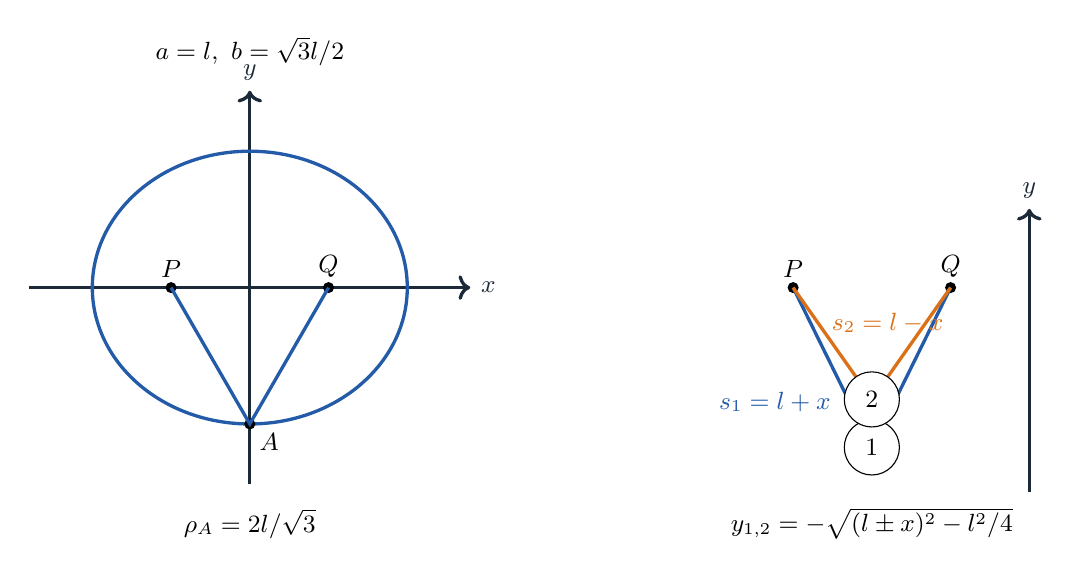
\begin{tikzpicture}[x=1cm,y=1cm,font=\small]

\begin{scope}[shift={(-3.9,0)}]
\draw[axis](-2.8,0)--(2.8,0)node[right]{$x$};\draw[axis](0,-2.5)--(0,2.5)node[above]{$y$};
\draw[curve](0,0)ellipse(2 and 1.732);\fill(-1,0)circle(2pt)node[above]{$P$};\fill(1,0)circle(2pt)node[above]{$Q$};
\coordinate(A)at(0,-1.732);\fill(A)circle(2pt)node[below right]{$A$};\draw[rope](-1,0)--(A)--(1,0);
\node at(0,3){$a=l,\ b=\sqrt3l/2$};\node at(0,-3){$\rho_A=2l/\sqrt3$};\end{scope}
\begin{scope}[shift={(4,0)}]
\fill(-1,0)circle(2pt)node[above]{$P$};\fill(1,0)circle(2pt)node[above]{$Q$};
\coordinate(M1)at(0,-2.03);\coordinate(M2)at(0,-1.42);
\draw[rope](-1,0)--(M1)--(1,0);\draw[very thick,orange](-1,0)--(M2)--(1,0);
\node[mass]at(M1){$1$};\node[mass]at(M2){$2$};
\draw[axis](2,-2.6)--(2,1)node[above]{$y$};
\node[blue,below left]at(-.4,-1.2){$s_1=l+x$};\node[orange,above]at(.2,-.7){$s_2=l-x$};
\node at(0,-3){$y_{1,2}=-\sqrt{(l\pm x)^2-l^2/4}$};\end{scope}
\end{tikzpicture}

% 5 question-03
\begin{tikzpicture}[x=1cm,y=1cm]
  \foreach \x in {-4.2,-3.4,...,4.2}
    \foreach \y in {-2.2,-1.4,...,2.2}
      {\node[ink!45] at (\x,\y) {$\otimes$};}
  \draw[very thick,orange] (-4,-1.7)--(4,1.7);
  \fill (0,0) circle (2.5pt) node[below right] {$O$};
  \node[mass] at (2.2,.94) {$q,\,2m$};
  \draw[force] (3.25,1.4) arc (20:82:1.25) node[above] {$\omega$};
  \draw[dim] (0,0)--(3.64,1.55) node[midway,above] {$l$};
  \node[above left] at (-3.7,2.25) {$\bm B$ 垂直纸面向里};
\end{tikzpicture}

% 6 solution-03
\begin{tikzpicture}[x=1cm,y=1cm,font=\small]

\begin{scope}[scale=2.6]
\draw[axis](-1.25,0)--(1.45,0)node[right]{$x/l$};\draw[axis](0,-.15)--(0,1.45)node[above]{$y/l$};
\draw[guide](-1,0)--(1,0);\node[below]at(1,0){释放点};
\draw[very thick,blue] plot coordinates {(1.000000,0.000000) (1.005123,0.014115) (1.009968,0.028328) (1.014532,0.042633) (1.018813,0.057026) (1.022810,0.071500) (1.026521,0.086050) (1.029945,0.100670) (1.033081,0.115355) (1.035927,0.130098) (1.038482,0.144895) (1.040745,0.159739) (1.042716,0.174625) (1.044393,0.189547) (1.045776,0.204499) (1.046864,0.219476) (1.047657,0.234471) (1.048155,0.249478) (1.048358,0.264493) (1.048264,0.279508) (1.047875,0.294519) (1.047191,0.309519) (1.046212,0.324503) (1.044937,0.339465) (1.043368,0.354398) (1.041506,0.369298) (1.039351,0.384158) (1.036903,0.398973) (1.034164,0.413737) (1.031135,0.428445) (1.027817,0.443089) (1.024212,0.457666) (1.020320,0.472168) (1.016143,0.486592) (1.011684,0.500930) (1.006942,0.515178) (1.001922,0.529329) (0.996623,0.543379) (0.991049,0.557322) (0.985202,0.571153) (0.979083,0.584865) (0.972696,0.598455) (0.966042,0.611916) (0.959124,0.625244) (0.951946,0.638432) (0.944509,0.651477) (0.936817,0.664373) (0.928872,0.677115) (0.920679,0.689698) (0.912238,0.702118) (0.903556,0.714368) (0.894633,0.726446) (0.885475,0.738345) (0.876084,0.750062) (0.866464,0.761592) (0.856619,0.772930) (0.846552,0.784072) (0.836269,0.795014) (0.825772,0.805751) (0.815065,0.816279) (0.804153,0.826594) (0.793041,0.836693) (0.781731,0.846571) (0.770230,0.856224) (0.758540,0.865649) (0.746667,0.874842) (0.734616,0.883800) (0.722390,0.892519) (0.709996,0.900995) (0.697436,0.909225) (0.684717,0.917207) (0.671844,0.924936) (0.658821,0.932411) (0.645653,0.939628) (0.632346,0.946584) (0.618904,0.953277) (0.605333,0.959704) (0.591638,0.965862) (0.577825,0.971750) (0.563898,0.977364) (0.549863,0.982704) (0.535727,0.987766) (0.521493,0.992548) (0.507167,0.997050) (0.492756,1.001268) (0.478265,1.005202) (0.463699,1.008850) (0.449064,1.012211) (0.434366,1.015282) (0.419610,1.018064) (0.404802,1.020555) (0.389948,1.022753) (0.375054,1.024659) (0.360125,1.026271) (0.345167,1.027589) (0.330186,1.028612) (0.315188,1.029340) (0.300178,1.029773) (0.285163,1.029909) (0.270148,1.029751) (0.255139,1.029297) (0.240142,1.028547) (0.225162,1.027502) (0.210206,1.026163) (0.195280,1.024529) (0.180388,1.022602) (0.165537,1.020382) (0.150733,1.017869) (0.135981,1.015066) (0.121287,1.011974) (0.106657,1.008592) (0.092097,1.004923) (0.077611,1.000968) (0.063206,0.996729) (0.048887,0.992206) (0.034660,0.987403) (0.020531,0.982321) (0.006504,0.976961) (-0.007414,0.971327) (-0.021219,0.965419) (-0.034905,0.959241) (-0.048467,0.952794) (-0.061899,0.946082) (-0.075196,0.939107) (-0.088354,0.931871) (-0.101366,0.924377) (-0.114228,0.916629) (-0.126936,0.908629) (-0.139483,0.900380) (-0.151866,0.891886) (-0.164078,0.883150) (-0.176117,0.874175) (-0.187976,0.864965) (-0.199652,0.855523) (-0.211140,0.845853) (-0.222435,0.835959) (-0.233533,0.825844) (-0.244430,0.815513) (-0.255121,0.804969) (-0.265603,0.794217) (-0.275871,0.783260) (-0.285921,0.772104) (-0.295749,0.760751) (-0.305353,0.749208) (-0.314727,0.737478) (-0.323868,0.725565) (-0.332773,0.713475) (-0.341438,0.701211) (-0.349860,0.688780) (-0.358036,0.676185) (-0.365962,0.663431) (-0.373636,0.650524) (-0.381053,0.637468) (-0.388213,0.624269) (-0.395111,0.610932) (-0.401745,0.597461) (-0.408113,0.583862) (-0.414212,0.570141) (-0.420039,0.556302) (-0.425593,0.542351)};
\draw[very thick,orange] plot coordinates {(0.617337,-0.786698) (-0.617337,0.786698)};
\fill (-0.425593,0.542351) circle(2pt) node[above left] {$P$};

\fill(0,0)circle(.8pt)node[below left]{$O$};\draw[vec](1,0)--(1.2,0)node[below]{$v$};\draw[vec](1,0)--(1,.38)node[right]{$\omega'l$};\end{scope}
\node[align=left,anchor=west]at(4,1.1){$\alpha=1$\\$\varphi_P=2.236$ rad\\$s_P/l=0.6894$\\$F'(\tau_P)=0.1631\ne0$};
\node at(1,-3.1){蓝色：自由小环；橙色：相交时的有限杆段};
\end{tikzpicture}

% 7 question-04
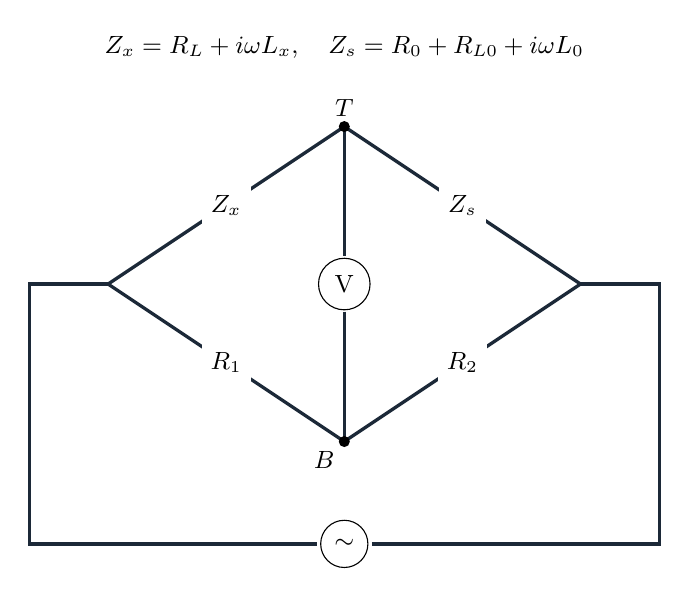
\begin{tikzpicture}[x=1cm,y=1cm,font=\small]

\coordinate(L)at(-3,0);\coordinate(R)at(3,0);\coordinate(T)at(0,2);\coordinate(B)at(0,-2);
\draw[body](L)--(T)--(R)--(B)--cycle;
\node[fill=white]at(-1.5,1){$Z_x$};\node[fill=white]at(1.5,1){$Z_s$};\node[fill=white]at(-1.5,-1){$R_1$};\node[fill=white]at(1.5,-1){$R_2$};
\draw[body](T)--(0,.35);\draw[body](0,-.35)--(B);\node[draw,circle]at(0,0){V};
\draw[body](L)--(-4,0)--(-4,-3.3)--(-.35,-3.3);\draw[body](.35,-3.3)--(4,-3.3)--(4,0)--(R);\node[draw,circle]at(0,-3.3){$\sim$};
\fill(T)circle(2pt)node[above]{$T$};\fill(B)circle(2pt)node[below left]{$B$};\node at(0,3){$Z_x=R_L+i\omega L_x,\quad Z_s=R_0+R_{L0}+i\omega L_0$};
\end{tikzpicture}

% 8 solution-04
\begin{tikzpicture}[x=1cm,y=1cm,font=\small]

\begin{scope}[shift={(-4.5,0)},scale=.75]
\coordinate(L)at(-3,0);\coordinate(R)at(3,0);\coordinate(T)at(0,2);\coordinate(B)at(0,-2);
\draw[body](L)--(T)--(R)--(B)--cycle;
\node[fill=white]at(-1.5,1){$Z_x$};\node[fill=white]at(1.5,1){$Z_s$};\node[fill=white]at(-1.5,-1){$R_1$};\node[fill=white]at(1.5,-1){$R_2$};
\draw[body](T)--(0,.35);\draw[body](0,-.35)--(B);\node[draw,circle]at(0,0){V};
\draw[body](L)--(-4,0)--(-4,-3.3)--(-.35,-3.3);\draw[body](.35,-3.3)--(4,-3.3)--(4,0)--(R);\node[draw,circle]at(0,-3.3){$\sim$};
\fill(T)circle(2pt)node[above]{$T$};\fill(B)circle(2pt)node[below left]{$B$};
\node at(0,3.1){$V_T=Uh(s),\ V_B=Ub$};\end{scope}
\begin{scope}[shift={(1,-2)}]
\draw[axis](0,0)--(6.3,0)node[right]{$n$};\draw[axis](0,0)--(0,4.5)node[above]{$\delta_n$};
\draw[very thick,blue] plot coordinates {(0.600000,3.767463) (1.200000,2.233531) (1.800000,1.453033) (2.400000,0.992713) (3.000000,0.698399) (3.600000,0.500705) (4.200000,0.363571) (4.800000,0.266342) (5.400000,0.196344) (6.000000,0.145399)};

\draw[red,dashed](0,.24)--(6,.24)node[right]{$0.03$};\fill[green](5.4,.1963)circle(2pt)node[above right]{9组};
\node at(2.8,-.8){误差分母：标称电感};\end{scope}
\end{tikzpicture}

% 9 question-05
\begin{tikzpicture}[x=1cm,y=1cm,font=\small]

\draw[body](-4,1.5)--(4,1.5);\draw[body](-4,-1.5)--(4,-1.5);
\node[above]at(0,1.5){$q_+=Q+CU$};\node[below]at(0,-1.5){$q_-=Q-CU$};
\draw[dim](-4.5,-1.5)--(-4.5,1.5)node[midway,left]{$x$};
\draw[guide](0,-1.5)--(0,1.5);\fill(0,0)circle(2pt)node[below left]{板轴};
\draw[body,orange](2.2,0)circle(.45);\draw[dim](0,-.75)--(2.2,-.75)node[midway,below]{$r$};
\node at(2.2,0){$\odot$};\node[right]at(3,0){$B_\varphi$，环法向};
\node at(0,-2.7){截面为径向—板法线平面；环在该竖直平面内};
\end{tikzpicture}

% 10 solution-05
\begin{tikzpicture}[x=1cm,y=1cm,font=\small]

\draw[axis](0,0)--(7,0)node[right]{$x/d$};\draw[axis](0,0)--(0,3)node[above]{$|\dot E|$（比例值）};
\draw[very thick,blue] plot coordinates {(0.000000,0.000000) (0.060606,0.421857) (0.121212,0.784733) (0.181818,1.097052) (0.242424,1.365897) (0.303030,1.597251) (0.363636,1.796188) (0.424242,1.967027) (0.484848,2.113453) (0.545455,2.238626) (0.606061,2.345260) (0.666667,2.435696) (0.727273,2.511957) (0.787879,2.575793) (0.848485,2.628727) (0.909091,2.672085) (0.969697,2.707023) (1.030303,2.734551) (1.090909,2.755556) (1.151515,2.770814) (1.212121,2.781010) (1.272727,2.786744) (1.333333,2.788548) (1.393939,2.786891) (1.454545,2.782187) (1.515152,2.774803) (1.575758,2.765066) (1.636364,2.753264) (1.696970,2.739653) (1.757576,2.724463) (1.818182,2.707896) (1.878788,2.690134) (1.939394,2.671337) (2.000000,2.651650) (2.060606,2.631201) (2.121212,2.610105) (2.181818,2.588463) (2.242424,2.566367) (2.303030,2.543899) (2.363636,2.521132) (2.424242,2.498130) (2.484848,2.474952) (2.545455,2.451649) (2.606061,2.428268) (2.666667,2.404850) (2.727273,2.381432) (2.787879,2.358046) (2.848485,2.334721) (2.909091,2.311484) (2.969697,2.288356) (3.030303,2.265359) (3.090909,2.242509) (3.151515,2.219822) (3.212121,2.197313) (3.272727,2.174993) (3.333333,2.152872) (3.393939,2.130959) (3.454545,2.109263) (3.515152,2.087789) (3.575758,2.066544) (3.636364,2.045531) (3.696970,2.024754) (3.757576,2.004217) (3.818182,1.983922) (3.878788,1.963870) (3.939394,1.944063) (4.000000,1.924501) (4.060606,1.905184) (4.121212,1.886113) (4.181818,1.867286) (4.242424,1.848703) (4.303030,1.830363) (4.363636,1.812264) (4.424242,1.794405) (4.484848,1.776783) (4.545455,1.759398) (4.606061,1.742246) (4.666667,1.725326) (4.727273,1.708635) (4.787879,1.692171) (4.848485,1.675931) (4.909091,1.659912) (4.969697,1.644112) (5.030303,1.628528) (5.090909,1.613158) (5.151515,1.597997) (5.212121,1.583045) (5.272727,1.568297) (5.333333,1.553751) (5.393939,1.539404) (5.454545,1.525253) (5.515152,1.511295) (5.575758,1.497528) (5.636364,1.483948) (5.696970,1.470553) (5.757576,1.457340) (5.818182,1.444306) (5.878788,1.431448) (5.939394,1.418763) (6.000000,1.406250)};

\draw[guide](1.333,0)--(1.333,2.789);\fill[green](1.333,2.789)circle(2pt)node[above]{$x/d=5/3$};
\node[below]at(0,0){1};\node at(3,-1){$B_\varphi=r|\dot E|/(2c^2)$};\node at(3,-1.7){峰值须处于忽略边缘场的近区};
\end{tikzpicture}

% 11 question-06
\begin{tikzpicture}[x=1cm,y=1cm]
  \coordinate (O) at (-4.2,0);
  \coordinate (P) at (4.2,0);
  \fill (O) circle (3pt); \fill (P) circle (3pt);
  \draw[very thick,blue]
    (O)..controls(-3.4,1.0)and(-2.8,-.9)..(-2.0,.35)
    ..controls(-1.3,1.5)and(-.5,-1.1)..(.3,.3)
    ..controls(1.1,1.25)and(2.1,-.8)..(2.9,.25)
    ..controls(3.35,.8)and(3.8,.45)..(P);
  \draw[dim] (O)--(P) node[midway,below] {$R$};
  \node[above left] at (O) {链首};
  \node[above right] at (P) {链尾};
  \node at (0,-1.65) {$N$ 个 Kuhn 链段，$\langle R^2\rangle=Nb^2$};
\end{tikzpicture}

% 12 solution-06
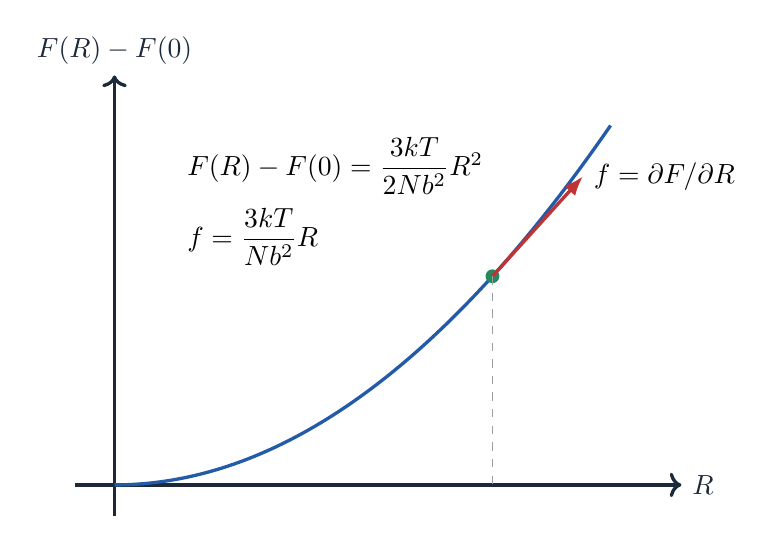
\begin{tikzpicture}[x=1cm,y=1cm]
  \draw[axis] (-.5,0)--(7.2,0) node[right] {$R$};
  \draw[axis] (0,-.4)--(0,5.2) node[above] {$F(R)-F(0)$};
  \draw[curve,domain=0:6.3,samples=80] plot (\x,{.115*\x*\x});
  \coordinate (T) at (4.8,{.115*4.8*4.8});
  \fill[green] (T) circle (2.5pt);
  \draw[force] (T)--++(1.15,1.27) node[right] {$f=\partial F/\partial R$};
  \draw[guide] (T)--(4.8,0);
  \node[align=left,anchor=west] at (.8,3.6)
    {$F(R)-F(0)=\dfrac{3kT}{2Nb^2}R^2$\\[4pt]
     $f=\dfrac{3kT}{Nb^2}R$};
\end{tikzpicture}

% 13 question-07
\begin{tikzpicture}[x=1cm,y=1cm,font=\small]

\draw[body](0,0)circle(2.5);\draw[body,fill=blue!8](1,.0)rectangle(1.6,.55);
\fill(0,0)circle(2pt)node[above left]{$O$};\draw[dim](0,-.35)--(1,-.35)node[midway,below]{$r$};
\draw[force](1,.275)--(2.45,.275)node[above right]{$p(r)A$};\draw[force](1.6,.275)--(.65,.275);\node at(-1.15,.6){$p(r+\mathrm dr)A$};
\draw[force](1.3,-.65)--(.4,-.65);\node[below]at(1.8,-1.2){$\rho A\mathrm dr\,g$ 向心};
\node[align=left]at(5,0){等温自引力气体\\$\rho=\mu p/(RT)$\\薄层压力沿径向};
\end{tikzpicture}

% 14 solution-07
\begin{tikzpicture}[x=1cm,y=1cm,font=\small]

\draw[axis](-3,0)--(3,0)node[right]{$r$};\draw[body](0,0)circle(1.5);\fill(0,0)circle(2pt)node[below]{$O$};
\fill(1.5,0)circle(2pt)node[above left]{$r_0$};\fill(2.1,0)circle(2pt)node[above right]{$r_0+\delta r$};
\draw[dim](1.5,-.6)--(2.1,-.6)node[midway,below]{$\delta r$};
\node[align=left,anchor=west]at(4,0){同一轨道的小径向扰动\\$\kappa^2=g_0/r_0+4\pi G\rho_0$\\$T_r=2\pi/\kappa$};
\end{tikzpicture}

% 15 question-08
\begin{tikzpicture}[x=1cm,y=1cm]
  \coordinate (O) at (0,0);
  \draw[axis] (-4.2,0)--(4.5,0) node[right] {$x$};
  \draw[axis] (0,-3.4)--(0,3.6) node[above] {$y$};
  \draw[body] (0,0) circle (2.65);
  \node[mass,minimum size=7mm] at (0,0) {$+Ne$};
  \foreach \a in {100,124,148,172}
    {\node[mass,minimum size=5mm,font=\scriptsize] at ({2.65*cos(\a)},{2.65*sin(\a)}) {$-$};}
  \coordinate (A) at ({2.65*cos(38)},{2.65*sin(38)});
  \coordinate (X) at (4,0);
  \node[mass,minimum size=6mm] at (A) {$-$};
  \draw[guide] (0,0)--(A);
  \pic[draw=ink,->,"$\theta$",angle radius=9mm,angle eccentricity=1.35]
    {angle=X--O--A};
  \draw[force] (-.460166,2.60974) arc (100:150:2.65) node[above left,yshift=9mm] {$\omega$};
  \draw[vec] (-3.7,-2.7)--(-1.65,-2.7) node[midway,above] {$S'\text{ 相对 }S:\ \beta c$};
\end{tikzpicture}

% 16 solution-08
\begin{tikzpicture}[x=1cm,y=1cm,font=\small]

\draw[axis](-2.8,0)--(3.2,0)node[right]{$x'$};\draw[axis](0,-2.5)--(0,2.8)node[above]{$y'$};
\draw[body](0,0)ellipse(1.6 and 2);\node[mass]at(0,0){$+Ne$};
\foreach\a in{20,60,100,140,180,220,260,300,340}{\node[blue]at({1.6*cos(\a)},{2*sin(\a)}){$-$};}
\draw[vec](0,-.3)--(0,-1.6)node[right]{$\boldsymbol p'$};\draw[vec](-1.6,0)--(-2.45,-.65)node[left]{$\boldsymbol u'$};
\node[align=left,anchor=west]at(4,.4){$t'=0:\ x'=r\cos\theta/\gamma$\\$\mathrm dN=\dfrac N{2\pi}(1+\beta a\sin\theta)\mathrm d\theta$\\$\mu_j'=\mu(1-\beta^2/2)$\\内禀磁化积分另用 $\mu_{\mathcal M}'$};
\end{tikzpicture}
\end{document}
